\documentclass[UTF8]{ctexart}
\usepackage[a4paper,left=3cm,right=3cm,top=2cm]{geometry}
\usepackage{amsmath}
\usepackage{enumitem}
\usepackage{float}
\usepackage{threeparttable}
\usepackage{caption}
\usepackage{multirow}
\usepackage{graphicx}


\setlength\lineskiplimit{5.25bp}
\setlength\lineskip{5.25bp}

\title{切变模量的测量——实验报告}
\author{崔士强 PB22151743}
\date{\today}

\bibliographystyle{plain}

\begin{document}

\maketitle

\section{实验目的}
本实验的目的是测量一段金属丝的切变模量
\section{实验原理}
对于一个半径为$R$,长度为$L$的圆柱体,固定其上端,转动下端,在弹性限度内,切变模量可表示为
\[G=\frac{2ML}{\pi R^4\varphi }\]
其中$M$为钢丝的恢复力矩,$\varphi$为扭转角.
若在金属丝下悬挂一圆盘,圆盘可自由转动,则有:
\[M=D\varphi\]
因此有:
\[G=\frac{2DL}{\pi R^4}\]
设圆盘转动惯量为$I_0$,则有:
\[M=I_0\frac{d^2\varphi}{dt^2}\]
解方程得:
\[T_0=2\pi \sqrt{\frac{I_0}{D}}\]
然而圆盘上的夹具导致转动惯量$I_0$难以直接测出,因此我们在圆盘上放置一个内半径为$r_\text{内}$,
外半径为$r_\text{外}$,质量为m的金属环,其转动惯量设为$I_1$,此时扭摆周期设为$T_1$,则有
\[I_1=\frac{1}{2}m\left(r_\text{内}^2+r_\text{外}^2\right)\]
\[T_1=2\pi \sqrt{\frac{I_0+I_1}{D}}\]
可以解出:
\[I_0=I_1\frac{T_0^2}{T_1^2-T_0^2}\]
\[D=\frac{2\pi^2m\left(r_\text{内}^2+r_\text{外}^2\right)}{T_1^2-T_0^2}\]
\[G=\frac{4\pi Lm\left(r_\text{内}^2+r_\text{外}^2\right)}{R^4\left(T_1^2-T_0^2\right)}\]
因此测出$T_1$, $T_0$, $m$, $L$, $R$, $r_\text{内}$, $r_\text{外}$这几个物理量即可得到
扭转模量$D$和切变模量$G$.
\section{实验装置}
本实验用到的仪器包括:支架,待测金属丝,圆盘,金属环,钢卷尺,游标卡尺,螺旋测微器,秒表. 
实验装置如图1所示.
\begin{figure}[h]
    \centering
    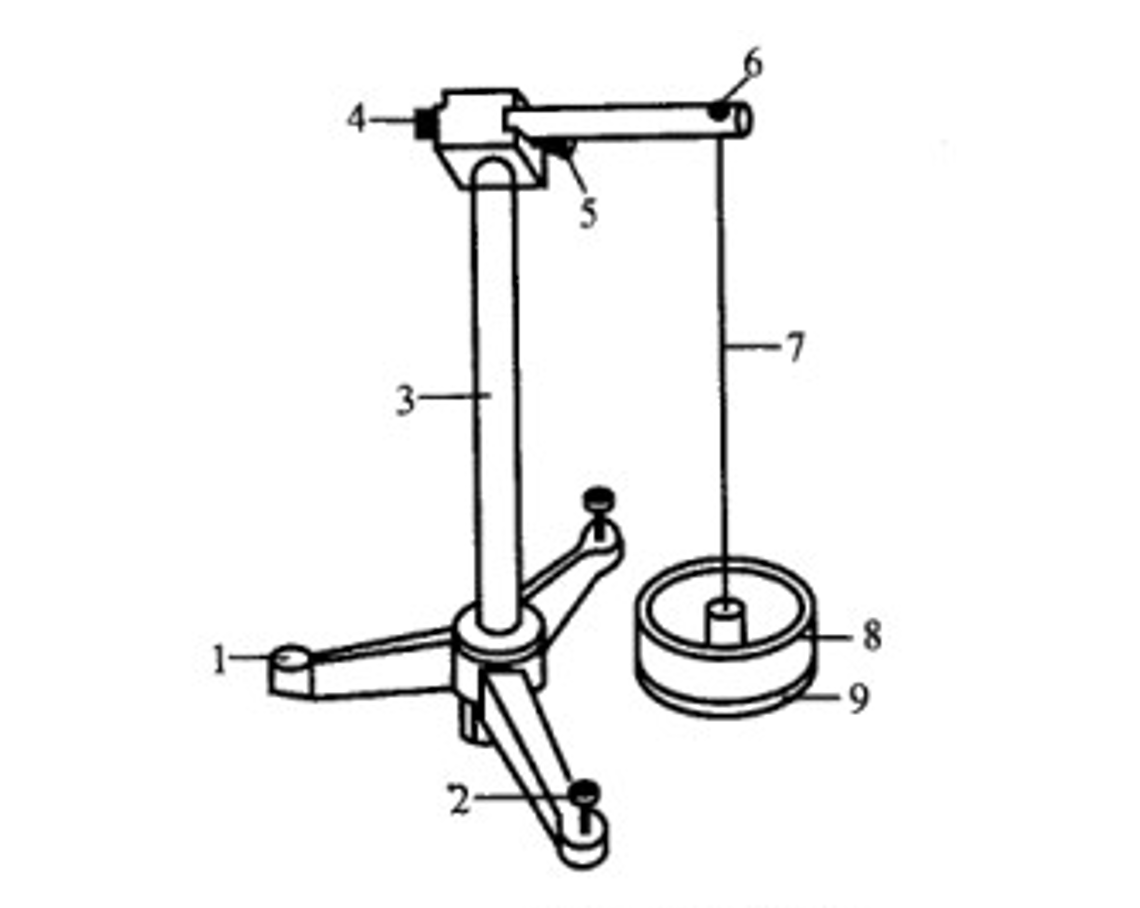
\includegraphics[scale=0.5]{装置.png}
    \caption{实验装置}
\end{figure}
\clearpage
\section{数据处理}
实验数据如下表所示
\begin{table}[H]\centering
    \begin{tabular}{ccccccc}
        \hline\hline
        $2R/mm$&$2r_\text{内}/mm$&$2r_\text{外}/mm$&$L/cm$&$m/g$&$n_0T_0/s$&$n_1T_1/s$\\
        \hline
        0.772&79.52&100&48.3&478.4&88.42&187.44\\
        0.771&79.72&100&48.28&478.4&88.58&187.51\\
        0.769&79.52&100&48.3&478.4&88.56&187.43\\
        0.768&79.76&100&48.3&478.4\\
        0.768&79.74&100&48.29&478.4\\
        0.768\\
        0.772\\
        0.776\\
        0.769\\
        0.768\\
        \hline\hline
    \end{tabular}
\end{table}
\begin{enumerate}
    \item 金属丝直径$d$
    \[\overline{d}=\frac{1}{10}\sum_{i = 1}^{10} d_i\approx 0.7701\mathrm{mm}\]
    \[\sigma _d=\sqrt{\frac{1}{n-1}\sum_{i=1}^{10}\left(d_i-\overline{d}\right)^2}\approx 0.002644\mathrm{mm}\] 
    \[\Delta_{B,d}=\sqrt{\Delta_{app}^2+\Delta_{est}^2}\approx \Delta_{app}=0.004\mathrm{mm}\]
    \[U_{d,P}=\sqrt{\left(t_P\frac{\sigma_d}{\sqrt{n}}\right)^2+\left(k_P\frac{\Delta_{B,d}}{C}\right)^2}\approx 3.4449\times 10^{-3}\mathrm{mm}, P=0.95\]
    \item 金属环内直径$d_\text{内}$
    \[\overline{d_\text{内}}=\frac{1}{5}\sum_{i = 1}^{5} d_{\text{内}i}\approx 79.652\mathrm{mm}\]
    \[\sigma _{d_\text{内}}=\sqrt{\frac{1}{n-1}\sum_{i=1}^{5}\left(d_{\text{内}i}-\overline{d}\right)^2}\approx 0.12133\mathrm{mm}\] 
    \[\Delta_{B,d}=\sqrt{\Delta_{app}^2+\Delta_{est}^2}\approx \Delta_{app}=0.02\mathrm{mm}\]
    \[U_{d_\text{内},P}=\sqrt{\left(t_P\frac{\sigma_{d_\text{内}}}{\sqrt{n}}\right)^2+\left(k_P\frac{\Delta_{B,d_\text{内}}}{C}\right)^2}\approx 0.15253\mathrm{mm}, P=0.95\]
    \item 金属环外直径$d_\text{外}$
    \[\overline{d_\text{外}}=\frac{1}{5}\sum_{i = 1}^{5} d_{\text{外}i}\approx 100.00\mathrm{mm}\]
    \[\sigma _{d_\text{外}}=\sqrt{\frac{1}{n-1}\sum_{i=1}^{5}\left(d_{\text{外}i}-\overline{d}\right)^2}=0\] 
    \[\Delta_{B,d}=\sqrt{\Delta_{app}^2+\Delta_{est}^2}\approx \Delta_{app}=0.02\mathrm{mm}\]
    \[U_{d_\text{外},P}=\sqrt{\left(t_P\frac{\sigma_{d_\text{外}}}{\sqrt{n}}\right)^2+\left(k_P\frac{\Delta_{B,d_\text{外}}}{C}\right)^2}\approx 0.022632\mathrm{mm}, P=0.95\]
    \item 钢丝长度$L$
    \[\overline{L}=\frac{1}{5}\sum_{i = 1}^{5} L_i\approx 48.294\mathrm{cm}\]
    \[\sigma _L=\sqrt{\frac{1}{n-1}\sum_{i=1}^{5}\left(L_i-\overline{L}\right)^2}\approx 0.008944\mathrm{cm}\] 
    \[\Delta_{B,L}=\sqrt{\Delta_{app}^2+\Delta_{est}^2}\approx \Delta_{app}=0.12\mathrm{cm}\]
    \[U_{L,P}=\sqrt{\left(t_P\frac{\sigma_L}{\sqrt{n}}\right)^2+\left(k_P\frac{\Delta_{B,L}}{C}\right)^2}\approx 0.07918\mathrm{cm}, P=0.95\]
    \item 圆环质量$m$
    \[\overline{m}=m=478.4\mathrm{g}\]
    \[\sigma _m=0\] 
    \[\Delta_{B,m}=\sqrt{\Delta_{app}^2+\Delta_{est}^2}\approx \Delta_{app}=0.08\mathrm{g}\]
    \[U_{m,P}=\sqrt{\left(t_P\frac{\sigma_m}{\sqrt{n}}\right)^2+\left(k_P\frac{\Delta_{B,m}}{C}\right)^2}\approx 0.05227\mathrm{g}, P=0.95\]
    \item $T_0$
    \[\overline{T_0}=\frac{1}{3}\sum_{i = 1}^{3} T_{0_i}\approx 2.5291\mathrm{s}\]
    \[\sigma _{T_0}=\sqrt{\frac{1}{n-1}\sum_{i=1}^{3}\left(T_{0_i}-\overline{T_0}\right)^2}\approx 0.002491\mathrm{s}\] 
    \[\Delta_{B,T_0}=\frac{1}{n_0}\sqrt{\Delta_{app}^2+\Delta_{est}^2}\approx \frac{1}{n_0}\Delta_{est}\approx 2.857\times 10^{-3}\mathrm{s}\]
    \[U_{T_0,P}=\sqrt{\left(t_P\frac{\sigma_{T_0}}{\sqrt{n}}\right)^2+\left(k_P\frac{\Delta_{B,T_0}}{C}\right)^2}\approx 3.6160\times 10^{-3}\mathrm{s}, P=0.95\]
    \item $T_1$
    \[\overline{T_1}=\frac{1}{3}\sum_{i = 1}^{3} T_{1_i}\approx 3.7492\mathrm{s}\]
    \[\sigma _{T_1}=\sqrt{\frac{1}{n-1}\sum_{i=1}^{3}\left(T_{1_i}-\overline{T_0}\right)^2}\approx 0.000872\mathrm{s}\] 
    \[\Delta_{B,T_1}=\frac{1}{n_1}\sqrt{\Delta_{app}^2+\Delta_{est}^2}\approx \frac{1}{n_1}\Delta_{est}\approx 2\times 10^{-3}\mathrm{s}\]
    \[U_{T_1,P}=\sqrt{\left(t_P\frac{\sigma_{T_1}}{\sqrt{n}}\right)^2+\left(k_P\frac{\Delta_{B,T_1}}{C}\right)^2}\approx 1.6978\times 10^{-3}\mathrm{s}, P=0.95\]
\end{enumerate}
扭转模量不确定度
\[U_D=\sqrt{\left(\frac{\partial D}{\partial m}U_{m,P}\right)^2+\left(\frac{\partial D}{\partial d_\text{内}}U_{d_\text{内},P}\right)^2+\left(\frac{\partial D}{\partial d_\text{外}}U_{d_\text{外},P}\right)^2+\left(\frac{\partial D}{\partial t1}U_{t1,P}\right)^2+\left(\frac{\partial D}{\partial t0}U_{t0,P}\right)^2}\]
代入数据得
\[U_D\approx 5.1728\times 10^{-5}\mathrm{Pa}, P=0.95\]
扭转模量
\[\hat{D}=\frac{\pi^2m\left(d_\text{内}^2+d_\text{外}^2\right)}{2\left(T_1^2-T_0^2\right)}\approx 6.7594\times 10^{-3}\mathrm{Pa}\]
扭转模量最终结果
\[D=\hat{D}\pm U_D=6.7594\times 10^{-3}\pm 5.1728\times 10^{-5}\mathrm{Pa}\]
切变模量不确定度
\begin{small}
    \[U_G=\sqrt{\left(\frac{\partial G}{\partial L}U_{L,P}\right)^2+\left(\frac{\partial G}{\partial m}U_{m,P}\right)^2+\left(\frac{\partial G}{\partial d_\text{内}}U_{d_\text{内},P}\right)^2+\left(\frac{\partial G}{\partial d_\text{外}}U_{d_\text{外},P}\right)^2+\left(\frac{\partial G}{\partial d}U_{d,P}\right)^2+\left(\frac{\partial G}{\partial t1}U_{t1,P}\right)^2+\left(\frac{\partial G}{\partial t0}U_{t0,P}\right)^2}\]
\end{small}
代入数据得
\[U_G\approx 2.8389\times 10^9\mathrm{Pa}\]
切变模量
\[\hat{G}=\frac{16\pi Lm\left(d_\text{内}^2+d_\text{外}^2\right)}{d^4\left(t_1^2-t_0^2\right)}\approx 9.45398\times 10^{10}\mathrm{Pa}\]
切变模量最终结果
\[G=\hat{G}\pm U_G=\left(9.45398\pm 0.28389\right)\times 10^{10}\mathrm{Pa}\]
相对不确定度为$3.0027\%$, 符合实验要求.
\section{思考题}
\begin{enumerate}
    \item 
    \[\gamma_{max}=R\frac{\varphi_{max}}{L} \approx 1.2524\times 10^{-3}\ll 1\]
    \item 采取的措施包括:测量多个周期求平均值,避免直接测量转动惯量等. 
    
    需要注意:放置圆环时,圆环重心需要与金属线重合. 测量金属丝长度时从上夹具下端到下夹具上端等.
\end{enumerate}

\bibliography{math}

\end{document}
\iffalse
\begin{figure}[h]
    \centering
    \includegraphics[scale=0.5]{name.png}
    \caption{name}
\end{figure}
\begin{table}[H]\centering
    \begin{tabular}{cccc}
        \hline\hline
        \multicolumn{2}{c}{钢卷尺}&\multicolumn{2}{c}{秒表}\\
        $\Delta_\text{仪}/cm$ & $\Delta_\text{估}/cm$ & $\Delta_\text{仪}/s$ & $\Delta_\text{估}/s$ \\
        \hline
        0.2&0.05&0.01&0.2\\
        \hline\hline
    \end{tabular}
    \caption{仪器的最大允差及估计误差}
\end{table}
\fi
